\documentclass[a4paper, 10pt, onecolumn]{report}

\usepackage[utf8]{inputenc}
\usepackage[OT1]{fontenc}
\usepackage[french]{babel}
\usepackage[dvipsnames, table]{xcolor}
\usepackage{graphicx}
\usepackage{fancyhdr}
\usepackage{calc}
\usepackage[a4paper,margin=2.5cm]{geometry}
\usepackage{array}
\usepackage{rotating}
\usepackage{hyperref}
\usepackage{makeidx}

\hypersetup{
colorlinks=true,
linkcolor=midnight,           
}

\makeindex

\begin{document}

\newcommand{\bold}[1]{\textbf{#1}}
\newcommand{\italic}[1]{\textit{#1}}
\newcommand{\surligne}[1]{\underline{#1}}
\newcommand{\couleur}[1]{\textcolor{#1}}
\newcommand{\maj}[1]{\textsc{#1}}
\newcommand{\machine}[1]{\texttt{#1}}
\newcommand{\be}{\begin{enumerate}}
\newcommand{\ee}{\end{enumerate}}
\newcommand{\bi}{\begin{itemize}}
\newcommand{\ei}{\end{itemize}}

\pagenumbering{arabic}
\xdefinecolor{midnight}{named}{MidnightBlue}
\pagestyle{fancy}
\fancyhf{}
\lhead{Riwan Blondé, André Dimitri et Quentin Dexheimer}
\rhead{\leftmark}
\rfoot{\thepage}
\lfoot{\italic{Licence Professionnelle ASRALL 2011-2012}}

\title{Configuration automatique d’un cluster de calcul avec Puppet}
\author{Riwan Blondé, André Dimitri et Quentin Dexheimer1}
\maketitle 
\clearpage

\tableofcontents

\chapter{Ennoncé du Projet Tuteuré}
\section{\couleur{midnight}{Le Sujet}}
L'énoncé tel que défini est le suivant : l’équipe devait réaliser une série de modules Puppet permettant de configurer un cluster de calcul 
de manière automatisée
\section{\couleur{midnight}{Le Travail Attendu}}
Le travail attendu consiste en un guide d’installation et d’utilisation de l’outil utilisé, des scripts permettant l’installation des modules 
puppet et de lancement de la configuration, plus une démonstration en temps réel sur la plate-forme Grid5000.
\section{\couleur{midnight}{Constitution d’un site Grid5000}}
Un site Grid5000 est constitué de plusieurs services : s’y trouvent un DNS, un serveur DHCP, une base de données MySQL ainsi que les outils de 
déploiement et de réservation OAR et kadeploy. S’y ajoutent également le service NFS, qui permet de stocker les dossier personnels d’utilisateurs.
Au niveau physique, un site géographique Grid5000 est représenté par une machine de frontend, plusieurs noeuds et les machines qui serviront 
pour le stockage NFS.

\chapter{La plate-forme Grid5000}
\section{\couleur{midnight}{Objectif de la création}}
L’objectif de la création de Grid5000 est d’atteindre 5000 processeurs sur les différents sites. Cela permettra d’avoir les moyens d’effectuer 
des recherches dans le domaine des grilles. Il sera ainsi possible d’effectuer des tests réels plutôt que de ne présenter que des résultats 
de simulation.

\section{\couleur{midnight}{Organisation}}
Grid5000 a vu le jour en 2003 suite au besoin exprimé par l’Etat Français de disposer d'une
grille informatique destinée à la recherche.\\
\\
Le projet Grid5000 est réparti sur différents sites qui sont interconnectés avec le réseau
Réseau National de télécommunications pour la Technologie l’Enseignement et la Recherche
(RENATER).\\
\\
Les sites sont composés de un ou plusieurs clusters, comme le site de Nancy avec Griffon et
Grelon. Chaque site est géré par son propre administrateur, ce qui entraîne une hétérogénéité
de configuration sur les différents sites. Par exemple, les frontends des différents sites qui ne
disposent pas des mêmes librairies.\\
\\
A l’heure actuelle, la plate-forme Grid5000 comporte au total 7244 coeurs,disponibles sur 1500
machines réparties sur les différents sites comme suit :
- Bordeaux : 154 machines
- Grenoble : 118 machines
- Lille : 100 machines
- Lyon : 135 machines
- Nancy : 92 machines
- Orsay : 340 machines
- Reims : 44 machines
- Rennes : 162 machines
- Sophia : 101 machines
- toulouse : 80 machines


\section{\couleur{midnight}{Les outils du Grid5000}}
\subsection{\couleur{gray}{OAR}}
OAR est une collection d’outils développée par le laboratoire IMAG1 de l’Institut National
de Recherche en Informatique et Automatique (INRIA) permettant de gérer un cluster de
machines. Il fonctionne avec Perl à l’aide de MySQL et prend en charge le mécanisme de
réservation ainsi que l’utilisation massivement simultanée des machines en cluster. Grid5000
fait partie des cinq partenaires de OAR.\\
\\
Lorsqu’un utilisateur souhaite accéder au projet depuis l’extérieur, il doit passer par une
machine pare-feu d’un des neufs sites de France, parmi celles qui acceptent ce genre de
connexion. Une fois ce pare-feu passé grâce à l’identification par clé SSH, c’est un frontal
qui s’offre à l’utilisateur. Celui-ci est pourvu d’un espace qui lui est dédié.\\
\\
Cet espace seretrouvera partout où l’utilisateur ira grâce à un montage Network File System (NFS), dans
n’importe quelle machine de n’importe quel cluster, tant qu’il ne quitte pas le site. En effet,
les espaces personnels ne sont pas encore partagés d’un site à l’autre, ce qui pose divers
problèmes d’harmonisation et de réplication des données. Sur ce frontal, les possibilités sont
très limitées et se cantonnent surtout à utiliser les outils OAR. \\
\\
La première chose que ces outils lui permettront de faire, c’est de réserver des nœuds. Dans le jargon des clusters, cela signifie
réserver un ensemble de machines physiques, pour pouvoir exécuter des actions dessus et
de façon parallèle. Une réservation se fait avec son nom d’utilisateur et pour un temps donné.\\
\\
Il est également possible de préciser le nombre de nœuds ou de processeurs souhaités. Par
le biais de filtres SQL, d’autres options sont offertes : réservation sur un cluster en particulier,
sélection de nœuds possédant un matériel spécifique, etc. Si la requête trouve les machines
correspondantes et que celles-ci sont libres dans l’intervalle de temps demandé, l’utilisateur est
automatiquement connecté sur la première des machines de sa réservation.
. L’environnement proposé par défaut est appelé l’environnement de développement. Celui-
ci lui permettra d’exécuter des programmes qui concerneront l’ensemble des machines de
sa réservation, auxquelles il peut accéder sans limite par SSH. Le principal intérêt de cet
environnement est d’exécuter des programmes MPI. Nous verrons cette norme par la suite,
mais retenez que c’est un moyen de faire travailler toutes les machines de la réservation en les
faisant communiquer facilement.\\
\\
Cet environnement de développement, différent sur chaque site et parfois même d’un cluster a
l’autre, est stocké sur une partition réservée sur chacun des nœuds. L’espace de l’utilisateur est
monté en NFS sur les nœuds réservés.


\subsection{\couleur{gray}{Kadeploy}}
Le déploiement consiste à installer son propre système d’exploitation sur tous les nœuds de la réservation. Dans ce cas, la réservation doit 
être prise en indiquant ses intentions lors de l’appel de la commande. Des systèmes préparés sont ensuite disponibles dans la base de données 
des sites (qui diffère d’un site à l’autre). \\
\\
Il est possible d’installer un de ces systèmes, de le copier-coller en ajoutant ou en supprimant des programmes, 
des données, et de compresser le tout pour en faire un environnement personnalisé, qui pourra être déployé sur une future réservation. Lorsque 
l’utilisateur réserve des nœuds pour un déploiement, il est redirigé vers un environnement spécial de déploiement sur le frontal. Il pourra alors 
demander le déploiement d’un système sur toutes les machines, qui redémarreront sur une partition différente après avoir effectué l’installation 
du système. Ce déploiement est géré principalement par kadeploy3, un outil également développé par l’INRIA.\\
\\
Pour constater le redémarrage de la machine et éventuellement détecter les problèmes qui peuvent survenir à cause de l’environnement, il est 
possible de visualiser directement la séquence de lancement du BIOS, avant même que le noyau Linux ne soit démarré. Kaconsole3 permet ceci, grâce à un 
contrôleur matériel et l’outil telnet.

\chapter{Le logiciel Puppet}
\section{\couleur{midnight}{Qu’est ce que Puppet Labs ?}}
uppet est un logiciel open source comportant les outils nécessaires à la configuration de
systèmes informatiques. Il est basé sur le langage de programmation Ruby , et est sous licence
GPL v2. Puppet a principalement été développé par Luke Kanies et son entreprise Puppet
Labs.\\
\\
Kanies a développé puppet grâce à son expérience dans les systèmes Unix et les systèmes
d’administration depuis 1997. Non satisfait des outils de configuration existants, il a commencé
à travailler avec des outils de développement en 2001, et a fondé Puppet Labs en 2005, une
entreprise de développement open source basée sur les outils d’automatisation. Peu de temps
après, Puppet Labs sort son nouveau produit phare : Puppet. Il peut être utilisé pour gérer la
configuration d’application sous Unix et OSX, mais aussi de Linux et Windows depuis peu de
temps.\\
\\
Son modèle est basé sur 3 piliers :
\be
	\item Le déploiement ,
	\item langage de configuration et une couche d’abstraction ,
	\item couche transactionnelle .
\ee

\section{\couleur{midnight}{Le Contexte}}
La gestion au quotidien des configurations systèmes et applicatives d’une entreprise représente
un travail très fastidieux. Puppet simplifie grandement la vie des administrateurs : plus de
contrôles et d’interventions à réaliser régulièrement. Puppet se charge d’imposer sur les
machines des utilisateurs les configurations « type » définies par l’administrateur. Puppet est un
outil de déploiement et de gestion centralisée de configurations pour les environnements Linux,
Unix et Windows ; les machines gérées pouvant être physiques ou virtualisées.

\section{\couleur{midnight}{Fonction principale}}
Puppet est un outil de déploiement et de gestion automatisés de configurations et de systèmes
informatiques (serveurs, postes de travail..). Il repose sur un modèle client/serveur : un serveur 
central sert de dépôt de configurations, les systèmes clients (nœuds) se mettant à jour de manière 
manuelle ou automatique.\\
\\
Avec Puppet, l’administrateur n’écrit pas un ensemble d’opérations à exécuter sur les différents
nœuds : sous la forme d’un script, l’administrateur décrit l'état final de la machine dans un
Manifest, ce qui l’affranchit de la connaissance des commandes propres à chaque système
d'exploitation pour arriver à cet état.\\
\\
Le client Puppet peut être exécuté à chaque fois, mais les
changements ne seront effectifs que si l'état de la machine ne correspond pas aux attentes de
l'utilisateur.

\chapter{Le travail réalisé}
\section{\couleur{midnight}{Choix techniques}}
Il a été décidé, d’après ce que nous dit l’énoncé, d’utiliser le logiciel de gestion centralisé
Puppet. Il existe deux raisons à cela : tout d’abord, nous connaissions le logiciel (par le biais
d’exposés techniques), d’autre part par sa grande simplicité de mise en oeuvre par le biais de
modules à rajouter.\\
\\
De plus, comme vous le verrez plus bas, les scripts ont été rédigés en langage Bash
et non Ruby, dans la mesure où nous n’avions pas encore les connaissances (et les cours) en
début de projet pour réaliser les scripts dans ce langage. Bash était également le langage le
plus utilisé entre les membres du projet.\\
\\
Nous avions comme contraintes d’installer les services cités en partie 1b. , ce qui
impliquait notamment de prendre en main les outils proposés commme OAR et Kadeploy.
Deux choix se sont offerts à nous concernant la gestion des ressources. Nous avons
préféré ne pas utiliser d’image de nos travaux, qui nous aurait simplifié la tâche mais qui n’était
pas forcément dans l’esprit du projet. Cela nous a permis également de repartir de machines
fraîchement installées et de pouvoir tester nos scripts sans avoir à désinstaller ce qui avait été
déjà fait avant tout test.

\section{\couleur{midnight}{État actuel des travaux.}}
\subsection{\couleur{gray}{Historique}}
Nous avons appris la première semaine à utiliser la plate-forme Grid5000 par le biais de
tutoriels.\\
\\
La deuxième semaine, nous avons pris en main Puppet pour une partie du groupe.
Nous avons réussi à installer manuellement l’intégralité d’une architecture Puppet (Master
Puppet + 2 clients) sur 3 noeuds réservés manuellement. En parallèle, un script de réservation
de machines, d’installation du maître Puppet et de l’installation des clients Puppet a été écrit.
Pour permettre d’utiliser Puppet, nous avons écrit des modules Puppet pour l’installation de la
base de données MySQL et d’un serveur D.N.S. \\
\\
La troisième semaine, nous avons continué la création de modules Puppet avec
l’écriture d’un module pour l’installation du N.F.S. . Nous avons également pris en main l’outil
de gestion de réseaux virtuels kavlan, et terminé les scripts automatiques de réservation des
noeuds (reserv.sh), ainsi que l'installation et configuration de Puppet sur le serveur Maître
Puppet et sur les clients Puppet.\\
\\
La quatrième semaine nous a permis d’inclure le module MySQL et de rédiger le rapport
de mi-projet.
\newpage
\subsection{\couleur{gray}{Scripts réalisés}}
\subsubsection{\couleur{orange}{Reserv.sh}}
Le premier script utilise l’architecture et les outils mis à disposition par la plate-forme
Grid5000 pour déployer un ensemble de noeuds sous distribution Debian.

\begin{figure}[htb]
\begin{center}
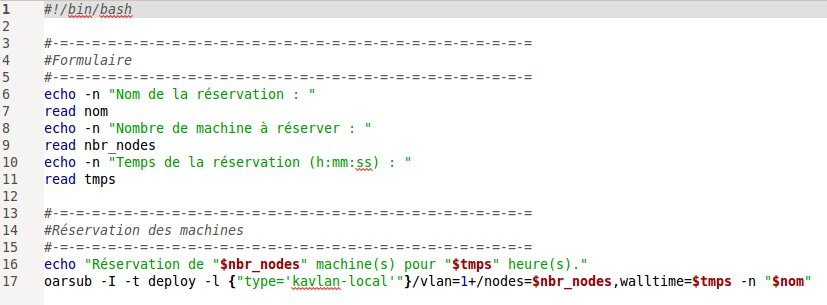
\includegraphics[scale=0.550]{images/reserv}
\caption{reserv}
\end{center}
\end{figure}


Nous avons décidé de simplifier la réservation en proposant un outil plus simple à prendre en
main dans la mesure où l’utilisateur n’a pas besoin de chercher dans les pages de manuel pour
apprendre la commande.

\subsubsection{\couleur{orange}{Install.sh}}

Intéressons nous maintenant au script le plus important, celui d’installation de l’ensemble des noeuds
réservés. 

\begin{figure}[htb]
\begin{center}
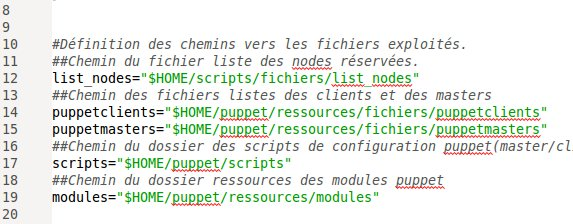
\includegraphics[scale=0.550]{images/install_1}
\caption{install part 1}
\end{center}
\end{figure}

Cette étape nous permet de personnaliser les chemins.

\newpage
Ici, une étape de mise en place du DHCP vlan pour le cluster, puis une vérification que l’utilisateur puisse 
bien se connecter via ssh aux nodes du vlan.

\begin{figure}[htb]
\begin{center}
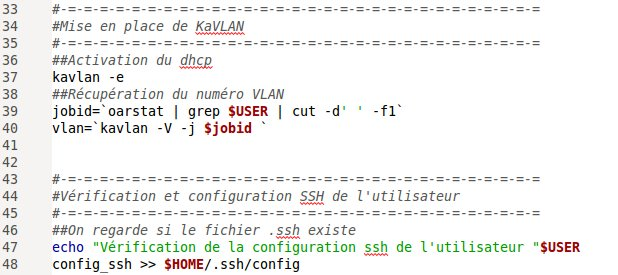
\includegraphics[scale=0.550]{images/install_2}
\caption{install part 2}
\end{center}
\end{figure}


Nous déployons les images disques sur les différents noeuds, puis nous créons les tunnels
SSH avec l’utilitaire taktuk fourni par Grid5000.\\
\\

\begin{figure}[htb]
\begin{center}
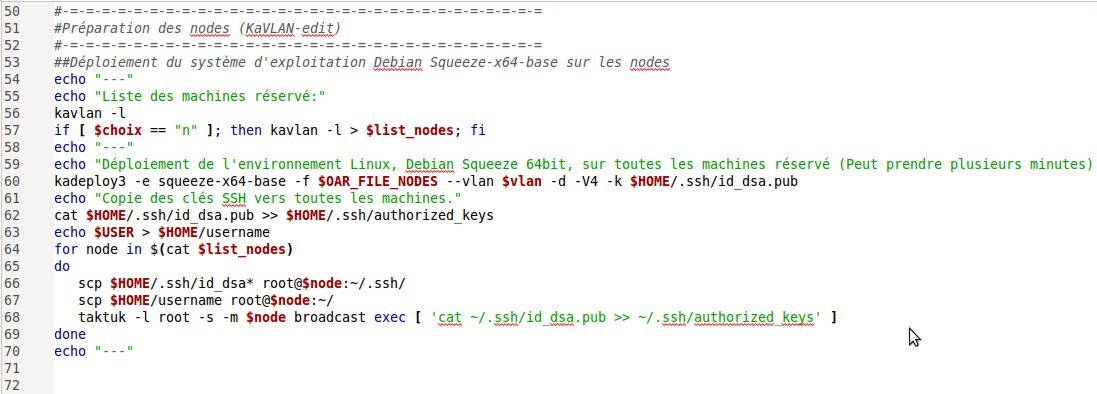
\includegraphics[scale=0.450]{images/install_3}
\caption{install part 3}
\end{center}
\end{figure}

Par la suite, nous installons ensuite la première machine en tant que Puppet Master, puis les
autres machines comme clients. \\
\\
\begin{figure}[htb]
\begin{center}
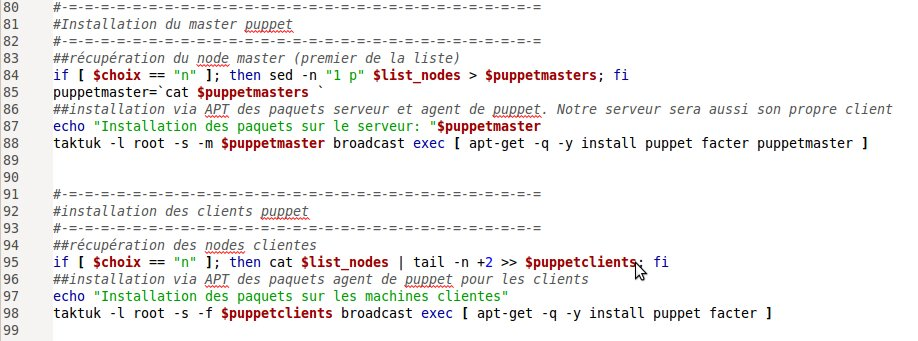
\includegraphics[scale=0.40]{images/install_4}
\caption{install part 4}
\end{center}
\end{figure}

Nous nous assurons enfin que les machines disposeront chacune d’un service avec Puppet.

\begin{figure}[htb]
\begin{center}
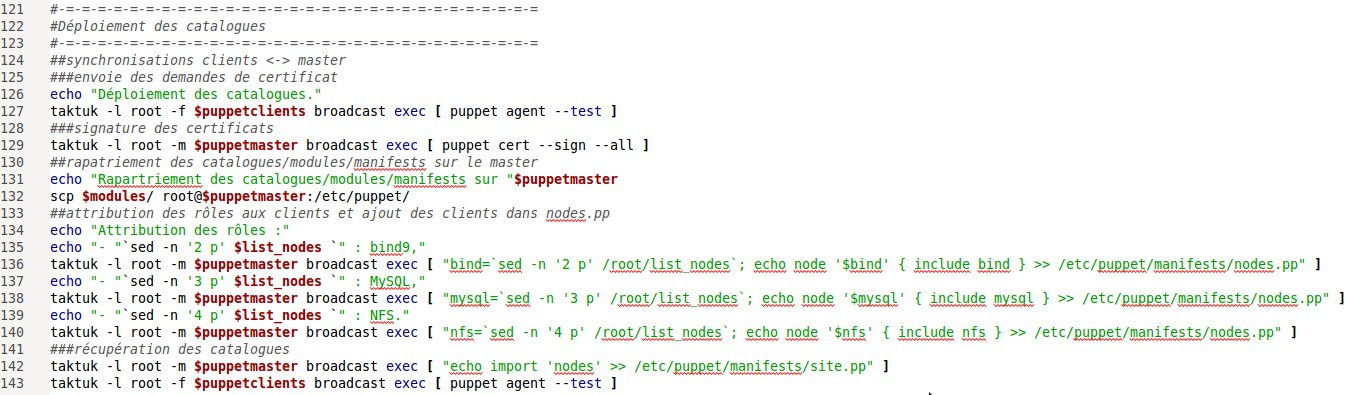
\includegraphics[scale=0.35]{images/install_5}
\caption{install part 5}
\end{center}
\end{figure}



\newpage
\subsection{\couleur{gray}{Poursuite du projet, ce qui est à venir...}}

A la moitié du projet, il nous reste encore beaucoup de tâches à réaliser. tout d’abord, il nous
reste à intégrer tous les modules comme le DNS, le DHCP, OAR et kadeploy. Il nous manquera
également une récupération de toutes les recettes Puppet afin de pouvoir consulter l’état des
machines. Lorsque toutes ces tâches seront réalisées, l’idéal serait de pouvoir installer un
Puppet Dashboard afin de pouvoir administrer l’intégralité des services en temps réel. Comparé
aux attentes du projet, nous réalisons déjà une installation sans image (en se basant tout de
même sur l’existant).




\end{document}